\documentclass[index]{subfiles}

\begin{document}
\title{Investigating the efficiency of Cheney stop-and-copy and LISP 2 style mark-compact garbage collection algorithms}
\date{}
\author{}
\maketitle

\section{Research Question}

How does a Cheney stop-and-copy algorithm compare to a LISP 2 mark-compact garbage collection algorithm in the context of a programming language? \cite{build_your_own_openjdk_gc}

\section{Introduction}

Garbage collectors, and the algorithms they use, are incredibly widespread in just about any application in modern day.

Higher level programming languages are a staple in the modern day. Javascript is the sole programming language of the web, and drives the functionality of all webpages. Python, the most popular programming language of today, still increasing in popularity over time and a language for first learners, Java, a still very popular programming language encodes Minecraft, one of the most popular games of the world, played by millions, and is used in tons of server-side applications worldwide.

The element that these programming languages all have in common is that they are interpreted languages, and they automatically manage memory, by using garbage collectors.

It thus follows that the algorithms behind garbage collection and their relative efficiencies are ever more important to consider, now that more interpreted languages are being run on more and more devices over time. Some recent studies on this subject have explored the power usages between different languages running the same program \cite{programming_languages_electricity}, comparing interpreted languages such as Java and Python with manually managed languages such as C++ and Rust, however, the results didn't specifically test garbage collection algorithms specifically, and as each language implements its own unique garbage collection algorithm with its own unique design decisions among other things, it's hard to say if one base garbage collection algorithm is better than the other using these results alone.

Other contemporary research on the subject has become increasingly complex, factoring in new algorithms, however, many assume the basic algorithms as known information, and haven't tested simple algorithms on modern hardware. This paper aims to shed light on the essential component of higher level languages that many programmers tend to look over, presenting information in an easily digestible way, as well as applying that knowledge practically by implementing a simple stop-and-copy and mark-compact garbage collection algorithm in the same programming language in an abstracted way, and comparing the performance of the two in this controlled environment.

\subsection{Methodology}

I will first do background research on basic terminology concerning memory management.

Then I will research how the two garbage collection algorithms are implemented, while attempting to create my own abstractions of the two algorithms in the Rust programming language.

I will then do research on the software and hardware factors in modern computers that garbage collection could have an effect on, including, but not limited to memory layout and algorithms that access the memory.

I will then consult 3 major papers that have compared the performances of these algorithms with others in the past.

I will then compare these views and add my own hypothesis on how the performance of the two algorithms might differ.

Finally, I will test both the collection performance of each algorithm (how long it takes to clean up the garbage) as well as the runtime performance of each algorithm, (such as accessing the data structure and its values during a traversal of the memory) using two separate tests.

\section{Background}

\subsection{The concepts of memory management (explained in the context of a game)}

\begin{quote}
    Imagine a game with multiple enemies. How do we store the enemies?
\end{quote}

The above question basically defines memory managment.

You might first think that a plain vector might take care of managing the enemies.

\begin{minted}[breaklines]{rust}
    enemies = [enemy1, enemy2, enemy3]
\end{minted}

Whenever you want to spawn an enemy, you \textit{allocate} it in the array

\begin{minted}[breaklines]{rust}
    enemies.push(enemy4)
    // enemies = [enemy1, enemy2, enemy3, enemy4]
\end{minted}

And whenever you want to despawn an enemy, you deallocate it from the array

\begin{minted}[breaklines]{rust}
    enemies.remove(0)
    // enemies = [enemy2, enemy3, enemy4]
\end{minted}

Simple enough, right?

But we're using some rather high-level abstractions here like \verb+remove+ and \verb+push+.

Imagine that the array you had was of a fixed length, and you couldn't push or pop from the array at will. Now how would you manage ``alive'' and ``dread'' enemies?

In this array, you would have to keep track of where the next free space was.

\begin{minted}[breaklines]{rust}
    free = 0
    enemies = [NULL, enemy2, enemy3]
\end{minted}

This simple action of keeping track of the free space, is where all the problems of memory management comes from.

\subsection{In the context of computers}

The data of all computer programs are stored in a place we call memory.

Whenever we want to make room for new data, we must allocate memory to free space. And whenever we want to remove data, we must deallocate that memory, back into free space.

In modern computers, there are two places where the program can allocate memory: the stack and the heap .

In the stack, whenever we wish to allocate something, all we have to do is bump a pointer's memory address up to determine where our next boundary of free memory is \cite{the_rust_programming_language}. However, whenever one wishes to deallocate memory, they must do so from top to the bottom.

Thus, the stack always consists of a block of contiguous used memory, and a block of contiguous free memory.

\begin{minted}[breaklines]{rust}
    free = 4
    memory = [data1, data2, data3, NULL, NULL, NULL]
\end{minted}

However, most of the memory of programs aren't allocated linearly and deallocated in the exact opposite order.

Thus, garbage collection is most concerned with the heap, which, on the other hand, can be accessed at random, and objects with dynamic sizes (that is, that is, sizes unknown at the time we compile our program) can be allocated on the heap. Deallocation of the heap may occur in a random order.

However, the question then becomes, how do we keep track of which sections of the heap are ``free'' memory, and which sections are ``used'' memory on the heap? That's the essence of memory managment.

\subsection{Memory Management Techniques}

There are several ways to manage memory in a language. One is by manually allocating and deallocating: the programmer specifies exactly how much memory is needed at a specific time, and decides when something should be deallocated. In lower-level languages, this is normal. However, manual allocation often requires a lot of experience to learn, and even with it, requires much more time to think about and write a program. It could also easily result in many types of bugs, such as using memory that is already freed, freeing memory twice, and not freeing memory in the first place \cite[Chapter~1]{garbage_collection_overview_uw, gc_handbook}

Hence, to alleviate the burden of having to keep track of manual memory management, many modern programming languages use automatic memory management. There are many different ways to automatically manage memory. The only types of garbage collectors this paper is concerned with are tracing garbage collectors, which, as their name suggests, directly check objects to determine if they are ``alive'' (used by the program) or ``dead'' (not in use any longer) \cite{a_unified_theory_of_garbage_collection}. In other words, tracing garbage collectors specifically determine if an object is accessible (garbage) or not by traversing some kind of tree \cite[Chapter~1]{gc_handbook}.

The main concept of garbage collection, simple: whenever we want to create a new object, we call \verb+allocate()+, and calculate the new free space on the heap. But if the heap is full, or if we wish to collect the garbage at any time, then we call \verb+collect()+ \cite{gc_handbook}, which as the name suggests, makes the bulk of the garbage collector.

\section{LISP 2 Sliding Mark-Compact Algorithm}

One very popular and easy to implement type of tracing garbage collector is the LISP 2 style mark-compact garbage collection algorithm.

\begin{figure}[H]
    \centering
    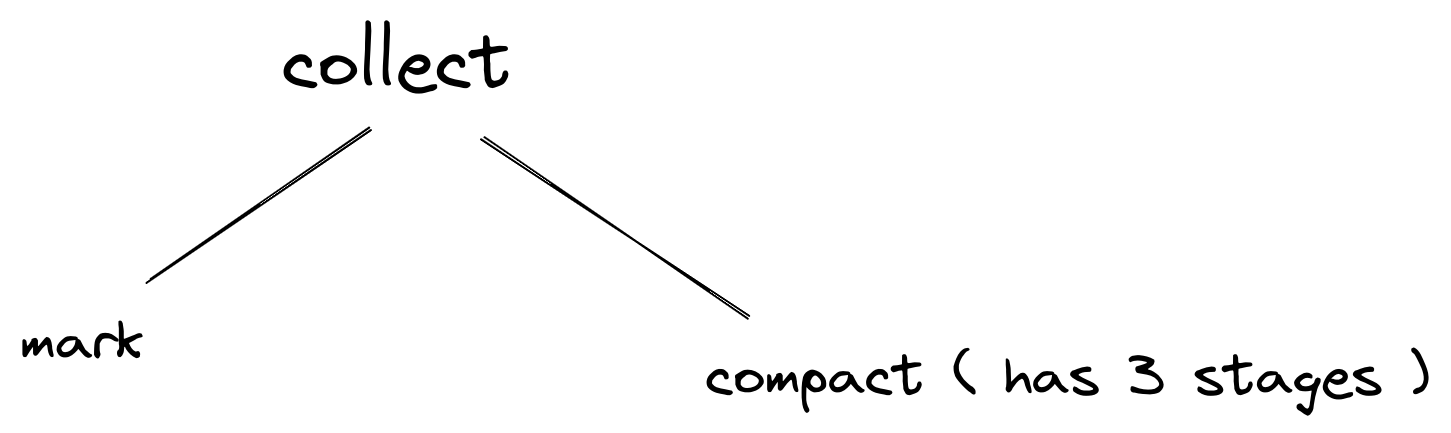
\includegraphics[scale=0.3]{pics/mark-compact-overview.png}
    \caption{Basic overview of mark-compact algorithm}
\end{figure}

The \verb+collect()+ function of this mark-compact algorithm can be broken down into two stages: the \verb+mark()+ stage, where we find out which objects are ``living'' and the \verb+compact()+ stage, where we perform a series of computations to ``slide'' the living objects down into one end, compacting the heap in the process and freeing up space \cite[Chapter~3]{gc_handbook}.

\subsection{The Marking Stage}

To determine which objects are alive and dead, we attempt to traverse the entire heap. We start from the root nodes, where the mutator can directly affect the values of the heap \cites[3.2~Marking]{redhat_openjdk}[Chapter~3]{gc_handbook}. Then we look at the objects that they reference. Accessible objects are objects that can eventually be reached by reference from the roots. We could use either breadth-first, or depth-first traversal to traverse the heap depending on the implementation, and  objects that are then found to be inaccessible (because they are unmarked) are defined as 'garbage', and can be removed in the next step, compaction.

\begin{minted}[linenos, breaklines]{rust}
// create marking bitmap using breadth-first traversal of the tree
let mut marked_node_pointers: BitVec = bitvec![0; self.committed_memory.len()];
{
    // first create a worklist, which is going to be a queue, since we're doing breadth-first traversal
    let mut worklist: VecDeque<NodePointer> = VecDeque::new();

    // populate the worklist with children from the reachable stack first
    for root in &stack.roots {
        for child in &root.children {
            worklist.push_back(*child);
        }
    }
    // then we just keep on taking from the worklist until it's empty
    while let Some(node) = worklist.pop_front() {
        // if the node isn't already marked
        if !marked_node_pointers[usize::from(node)] {
            // we mark it because it means it's accessible
            marked_node_pointers.set(usize::from(node), true);
            // then add the rest of its children to the back of the queue
            for child_node_pointer in &self.get(node).unwrap().children {
                worklist.push_back(*child_node_pointer);
            }
        }
    }
}
// now all our reachable objects should be marked, everything not in the list is garbo
\end{minted}

As for storing whether an object is marked with a starting bit, a rather expensive but easy to implement option is to use a bitmap (an array of bits, basically) where each index corresponds to each object in the heap, which is marked 1 or 0 to show that it is alive (1) or dead (0) \cite[Chapter~3]{gc_handbook}.

\subsection{Compact Stage}

The compaction stage of the mark-compact algorithm can be broken down into three parts, and in each part, the heap is traversed in its entirety. The first stage is to calculate the location of where the living object will slide down after copying. We do this by initializing a \verb+free+ pointer starting at the very bottom of the heap, and set the \verb+forwarding_address+ of the living marked object in question to the free pointer, then bumping its size up \cites[Chapter~3]{gc_handbook}[Sections~3.3-3.5]{redhat_openjdk}.

\begin{minted}[linenos, breaklines]{rust}
// free starts at 0, the beginning of the point which we wish to compact to
let mut free = 0;
// compact occurs next
{
    // the first step is to calculate new locations of all objects

    // we iterate over all objects in the heap TODO vec of nodes seems really inefficient
    // if it is marked,
    iterator.clone().try_for_each(|(idx, _)| -> Result<()> {
        let mut marked_node = self.get_mut(NodePointer::from(idx)).unwrap();
        // set its forwarding address equal to free
        marked_node.forwarding_address = Some(NodePointer::from(free));
        // then bump free
        free += 1;
        if free > self.committed_memory.len() {
            Err("not enough space on heap to allocate new object. Something went wrong with marking objects in `collect()`".into())
        } else {
            Ok(())
        }
    })?;
}
\end{minted}

The second stage of garbage collection is to update the references of each marked living object to point to the new \verb+forwarding_address+ of where they'll eventually be moved. We do this by traversing the heap for a 2nd time, then checking the reference of each object, retrieving the \verb+forwarding_address+ and setting that as the new reference on the object \cites[Chapter 3]{gc_handbook}[Sec. 3.4]{redhat_openjdk}.

\begin{figure}[H]
    \centering
    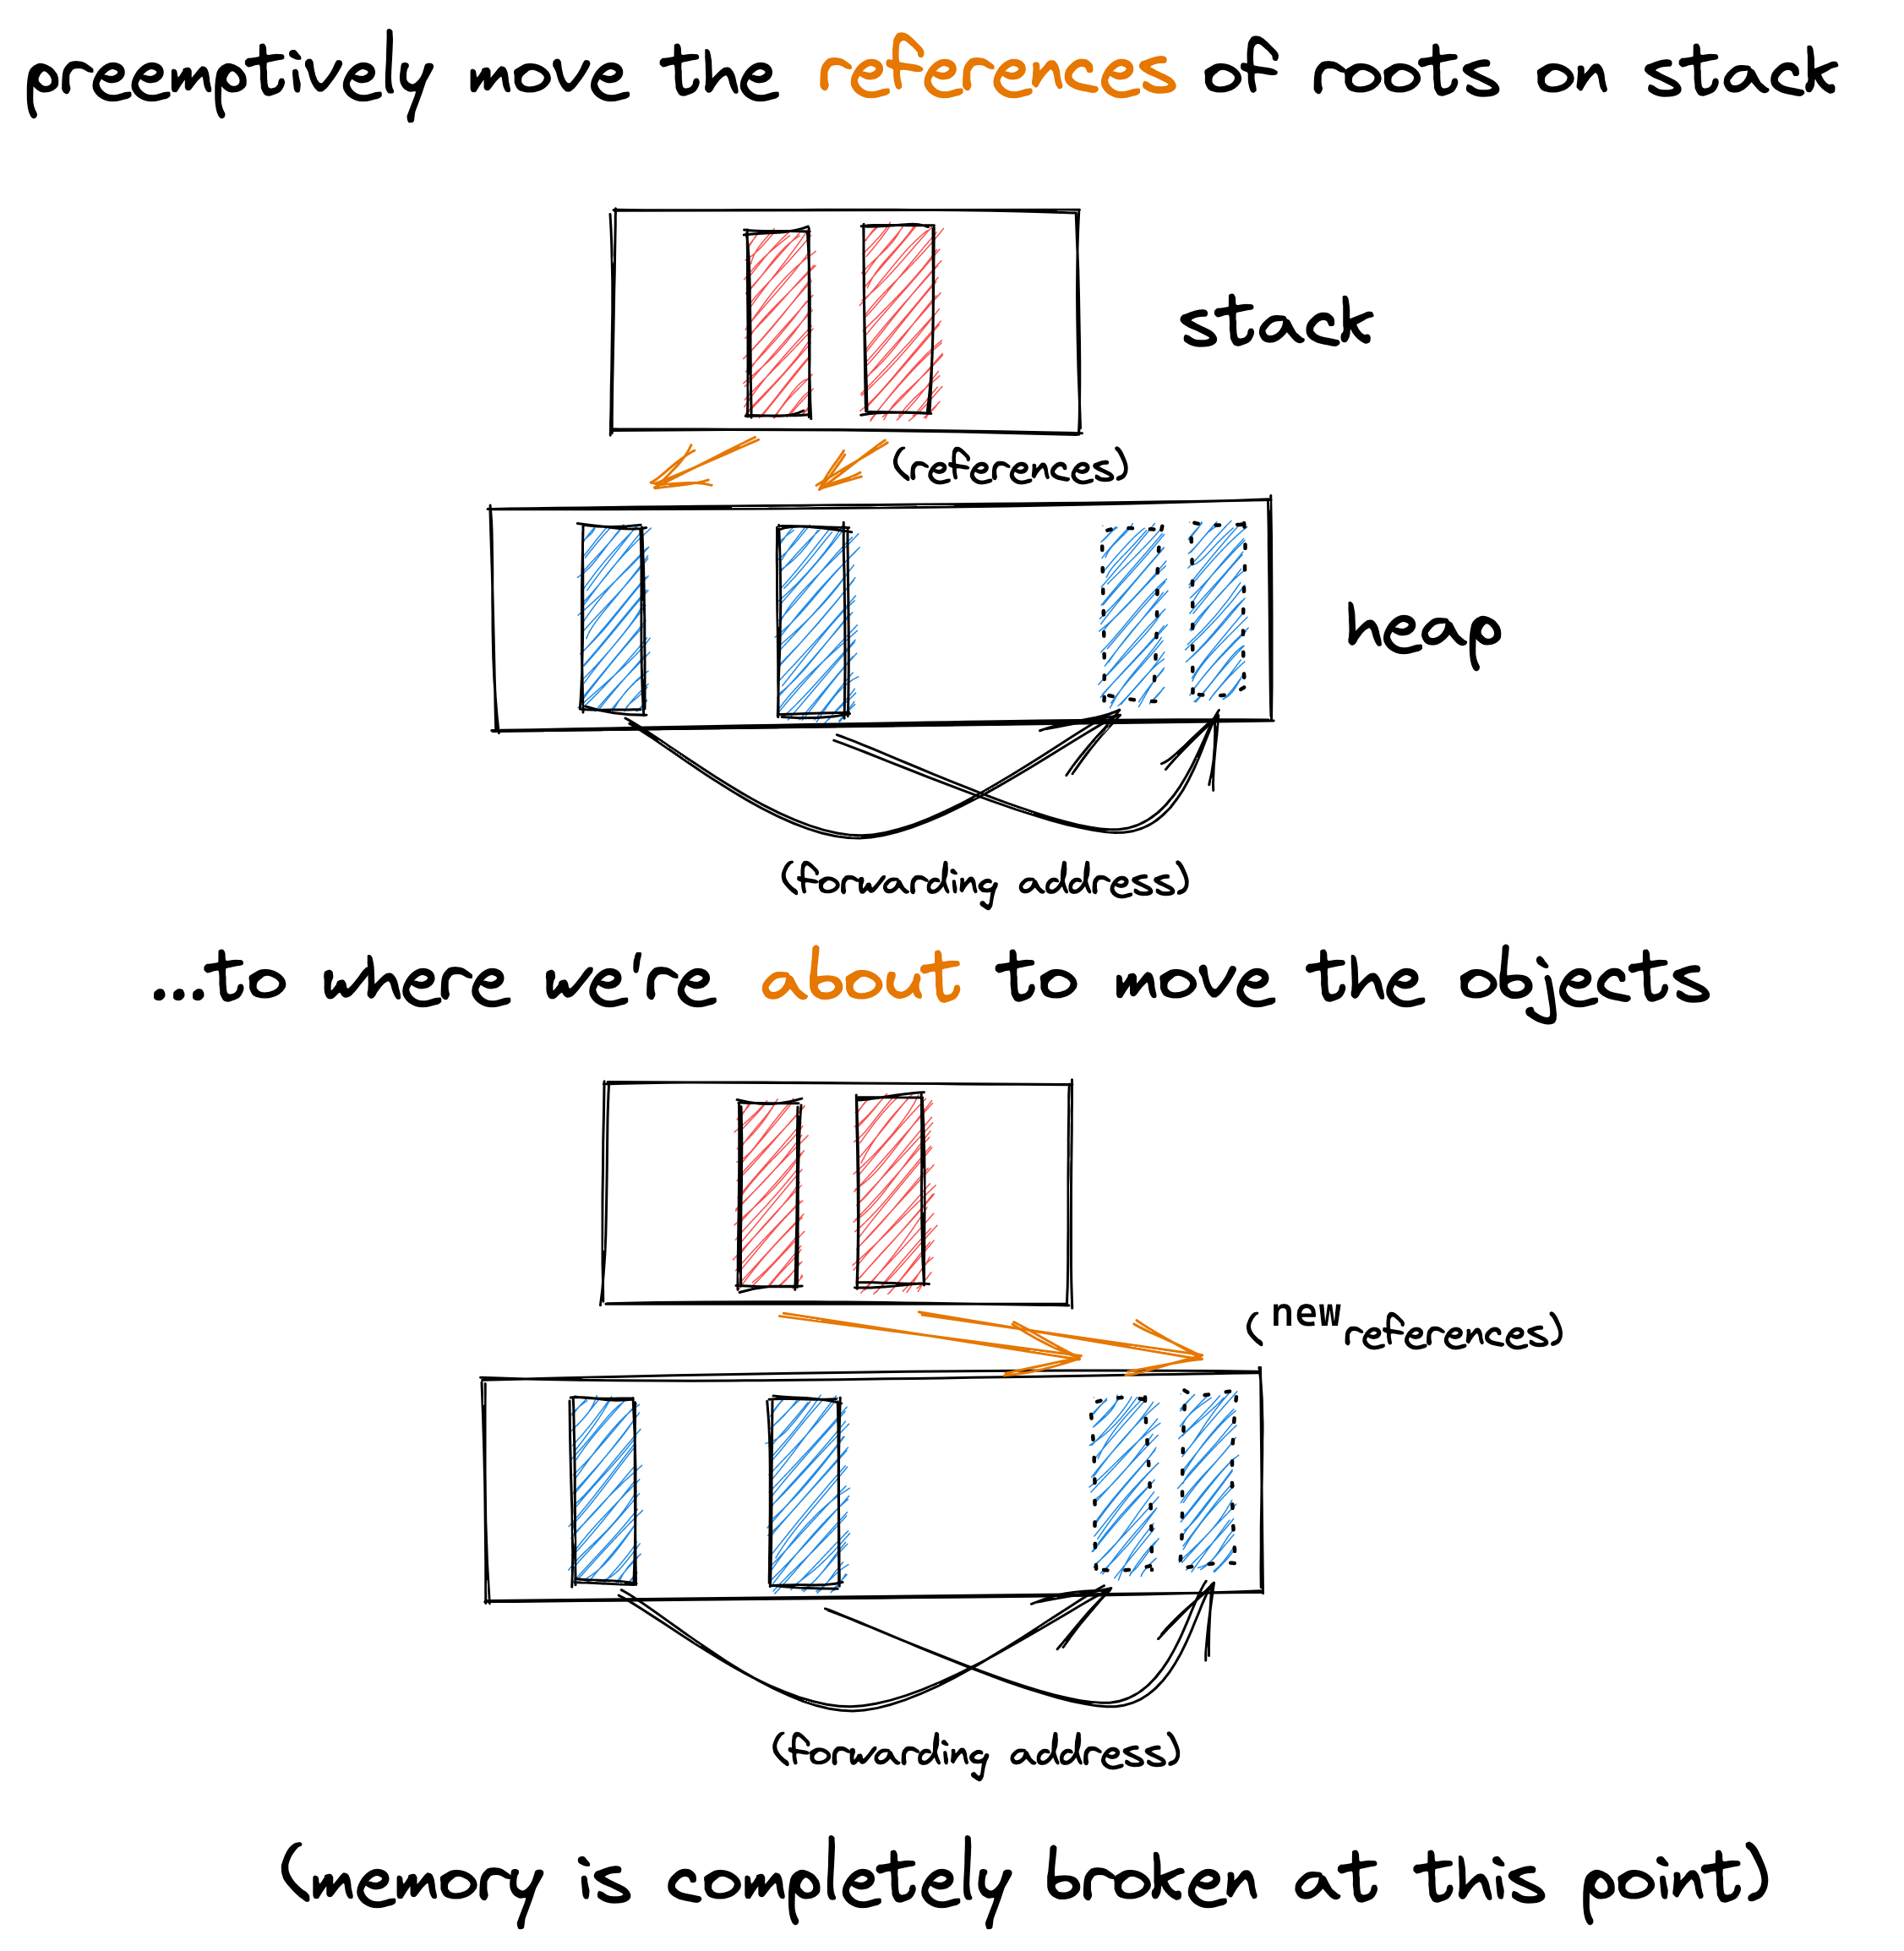
\includegraphics[scale=0.3]{pics/update-references.png}
    \caption{Updating references in the compact step of mark compact, visualized.}
\end{figure}

We know where the objects should and will point, because in the previous step we stored them in the objects \verb+forwarding_address+ field.

Finally, we can actually move the objects over to where their \verb+forwarding_address+ points to

\begin{figure}[H]
    \centering
    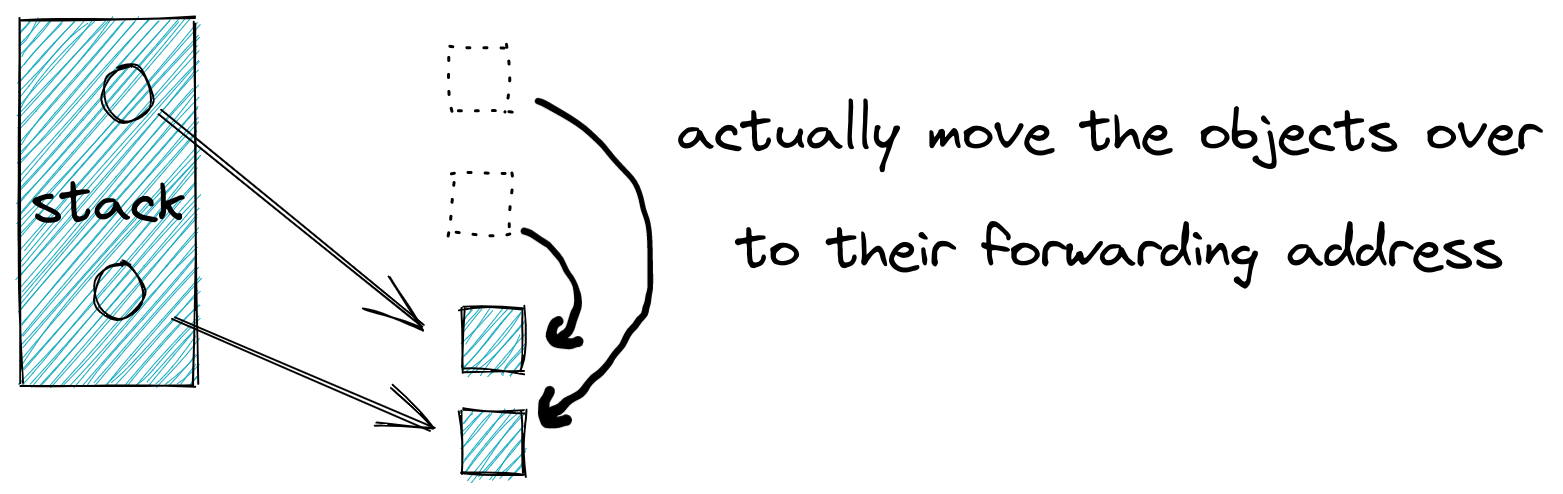
\includegraphics[scale=0.3]{pics/actually-move.png}
    \caption{Actually moving objects, the "compact step" in the compact step of mark compact, visualized.}
\end{figure}

We do this by traversing the heap a third time, then just doing some \mintinline{rust}{std::mem::swap} calls between the object's pointer and their forwarding address. It's important to note here, that the sliding mark-compaction algorithm maintains the order of which the objects were on in the original heap, as well as moves objects more closely together in memory, hence 'compacted.'

The order is important in the comparison between mark-compact and stop-copy garbage collection algorithms, because as we'll soon see, LISP 2 style stop-copy collectors do not preserve the order of objects in memory.

\subsubsection{Side note on page}

In most modern computers, including Windows and Linux, memory in a program is virtual memory, and each range of virtual memory maps to a range of physical memory addresses on hardware \cite{code_project}. These are stored in tables, and there is a \verb+page+ storage allocated for each address in order to link these virtual addresses to physical addresses. However, looking up these values is actually fairly expensive in terms of performance, so physical hardware has a lookup cache, with around the last 500 pages stored in it. Therefore, when objects are closer together in memory or when the order is maintained, it might provide a locality bonus, therefore increasing performance. However, it is still important to note that this implementation still traverses the heap itself 3 times in order to compact objects, which would be a fairly expensive thing to do on large heaps.

\section{Cheney's Stop-and-Copy Algorithm}

The second type of garbage collector that is of relevance to this paper is the stop-and-copy algorithm, which uses double the memory of the mark-compact compact algorithm, but is able to compress objects without walking them multiple times.

When initializing the heap using this algorithm, the initial contiguous heap is split into two sections, a \verb+from_space+ and a \verb+to_space+.

\begin{figure}[H]
    \centering
    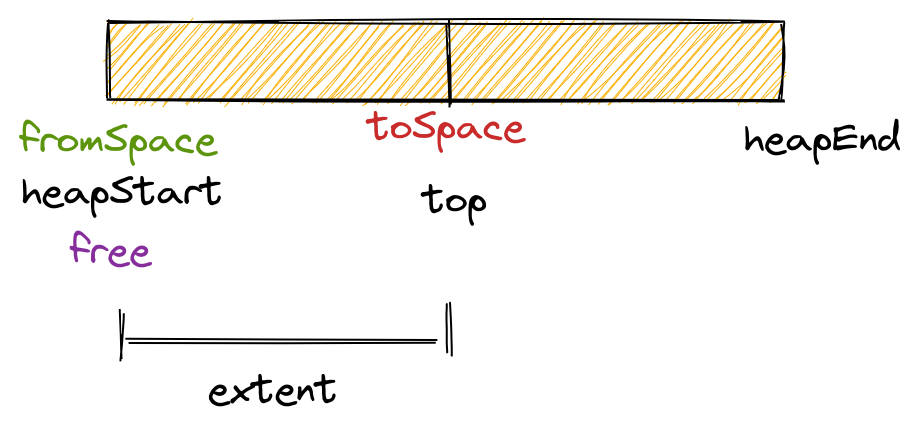
\includegraphics[scale=0.3]{pics/split-heap-diagram.png}
    \caption{Picture of what the heap looks like for stop and copy}
\end{figure}

Like other garbage collectors, on every allocation it asks if the heap has enough memory

\begin{figure}[H]
    \centering
    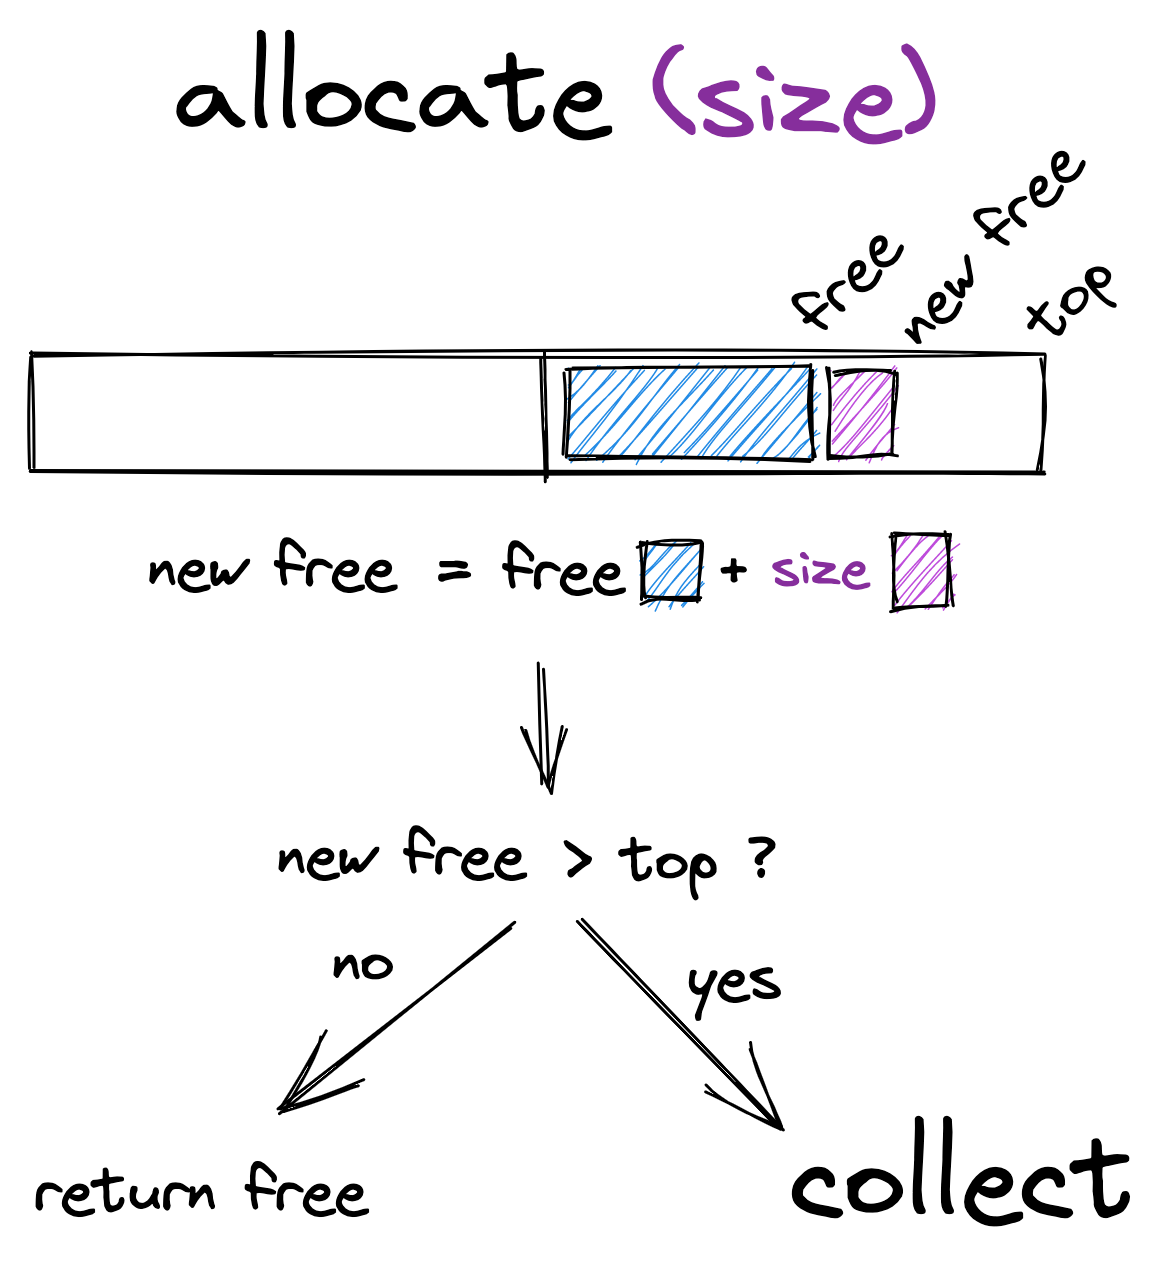
\includegraphics[scale=0.3]{pics/allocation.png}
    \caption{What checking for allocations looks like.}
\end{figure}

\begin{minted}[linenos, breaklines]{rust}
// allocates a new node
// we can just add a new node and return its id
fn alloc(&mut self, node: Node, stack: &mut Stack) -> Result<NodePointer> {
    // check if free is going over fromspace + tospace
    if self.free >= self.top {
        log::trace!("exceeded from space, must run garbage collector");
        // we need to run gc
        self.collect(stack)?;
    }
    if self.free >= self.top {
        return Err("gg collection didn't result in any amount of garbage collected".into());
    }

    // set the node id to where the top of the heap is
    let node_pointer = NodePointer::from(self.free);
    // add it to the heap
    self.committed_memory[usize::from(node_pointer)] = node;
    // bump the free pointer
    self.free += 1;

    Ok(node_pointer)
}
\end{minted}

In this case, because the heap is split in half, we check that the \verb+free+ is not greater than the end of the heap but rather that it is not greater than half of the size of the heap. Once the heap does end up filling up, we can no longer allocate a new object on the heap and thus must call the \verb+collect()+ function of the stop-and-copy garbage collection algorithm.

\subsection{Cheney's Algorithm}

Right as we jump into the collect function, we flip the \verb+from_space+ with \verb+`to_space`+.


\begin{minted}[linenos, breaklines]{rust}
    // first we swap from space with tospace
{
    std::mem::swap(&mut self.from_space, &mut self.to_space);
    // set free to be at the bot of the new to_space
    self.free = self.to_space;
    // set top to be to_space plus the extent
    self.top = self.to_space + self.extent;
}
\end{minted}

\begin{figure}[H]
    \centering
    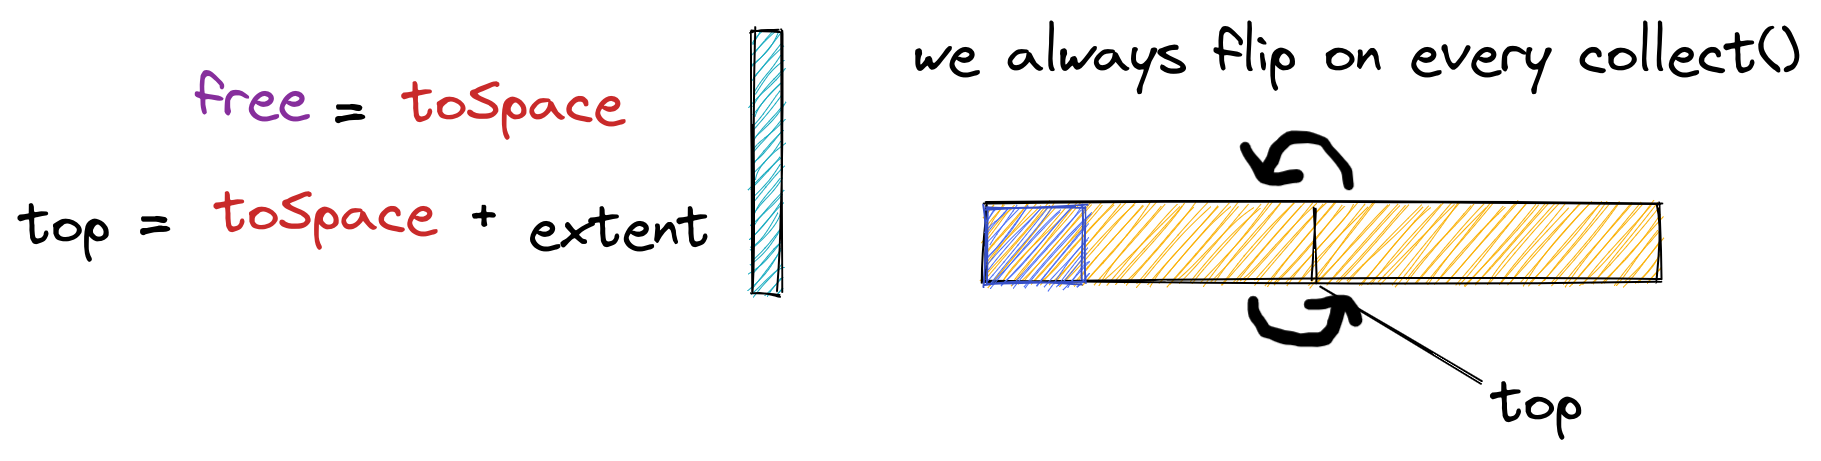
\includegraphics[scale=0.3]{pics/flipping.png}
    \caption{flipping}
\end{figure}

Then we follow that by moving the initial nodes accessible by the global mutator to space, with their original references in the \verb+from_space+ still pointing towards the old references.

\begin{minted}[linenos, breaklines]{rust}
// next we populate the initial "working list" with roots
{
    // copy the roots over
    // this technically adds them to the worklist
    for root in &mut stack.roots {
        for child in &mut root.children {
            // make sure to update the root refs to point in the right place
            *child = self.copy(*child)?;
        }
    }
}
\end{minted}

We update the \verb+forwarding_address+ of their old location on \verb+from_space+ to point to their new location on \verb+to_space+, via the \verb+copy+ function.

\begin{minted}[linenos, breaklines]{rust}
/// copy function
pub fn copy(&mut self, node_pointer: NodePointer) -> Result<NodePointer> {
    // if object has a forwarding address, it means that we've already moved it over to to space, so we can just give it its reference
    if let Some(forwarding_address) = self.get(node_pointer).unwrap().forwarding_address {
        Ok(forwarding_address)
    } else {
        let new_node_pointer = NodePointer::from(self.free);
        // otherwise, the new nodepointer value of this object will be whatever free there is
        // now use .swap() to move nodepointer current location to its new location free
        self.committed_memory
            .swap(usize::from(node_pointer), usize::from(new_node_pointer));

        // and remember to set the forwarding address of the moved nodepointer to none
        self.get_mut(new_node_pointer).unwrap().forwarding_address = None;

        // now update the old forwarding address to include itself
        // keep in mind that this object in to space is complete garbage except for the forwarding address part
        self.get_mut(node_pointer).unwrap().forwarding_address = Some(new_node_pointer);

        // also remember to bump free
        self.free += 1;

        // finally we can return the new_node_pointer
        Ok(new_node_pointer)
    }
}
\end{minted}

\begin{figure}[H]
    \centering
    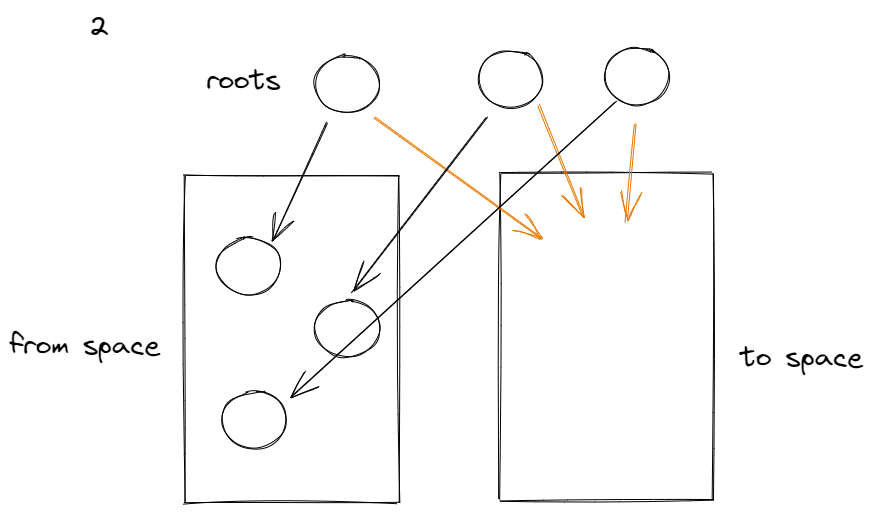
\includegraphics[scale=0.3]{pics/visualization-of-worklist.png}
    \caption{The algorithm for stop and compact. Unlike mark compact, instead of traversing the heap 3 times, it only traverses the heap once.}
\end{figure}

Now, we don't even need a worklist! Instead, we just repeatedly iterate over the objects in \verb+to_space+, until we reach the end of all the objects in \verb+to_space+. For every object that we then encounter (including the roots that we just moved), we find their references, move them over to \verb+to_space+ if we haven't already, and then update the references to point to \verb+to_space+. (If their references have already been moved, then we can just use their \verb+forwarding_address+ that we updated on the \verb+from_space+ to point to the right location).

\begin{minted}[linenos, breaklines]{rust}
    // now we process all the references of the nodes in the worklist as well
{
    // you might be wondering...
    // how do we do `for each node in worklist`?
    //
    // well, so long as the scan does not catch up to free
    // that is, so as long as we have not processed every single "copied" oject on the heap, keep on going
    while scan < self.free {
        let scan_node_pointer = NodePointer::from(scan);
        // get all references, or children of the object that was recently copied to tospace
        //
        //
        //  ... to copy the references over,
        for i in 0..self.get(scan_node_pointer).unwrap().children.len() {
            // set the reference to whatever the forwarding address stored inside the reference is, or copy it
            //
            // TL;DR the reference should now be pointing to copied objects in the tospace no matter what
            self.get_mut(scan_node_pointer).unwrap().children[i] =
                self.copy(self.get(scan_node_pointer).unwrap().children[i])?;
            // the references get added to the worklist automatically
        }
        // don't forget to bump the scan pointer
        scan += 1;
    }
}
\end{minted}

Upon reaching the end of the \verb+to_space+, garbage collection is already done! At this point the from-space is basically ignored, and the \verb+to_space+ becomes the effective heap, until the next cycle of garbage collection occurs.

However, despite the fact that Cheney's stop-and-copy algorithm has much fewer steps than the mark-compact garbage collector, it has several downsides. Apart from the most obvious thing being the heap split in half, it's important to note that the way the worklist is traversed in this algorithm, it's effectively breadth-first by reference. Therefore, when objects are moved, their original order is not preserved, unlike with the mark-compact garbage collector. This could negatively affect program performance, because parents have the possibility of being separated from their children, resulting in large differences in locality despite the heap being compacted.

It should be noted that mark-and-compact and stop-and-copy garbage collectors are also both moving garbage collectors, meaning that memory is swapped and copied around throughout the garbage collection cycle. Moving large surviving objects multiple times will inevitably lead to poor performance \cite[Chapter 4]{gc_handbook}.

Stop-and-copy garbage collection actually moves more than mark-compact garbage collection, because there isn't the possibility of objects staying in place and already being compacted. But on the flipside, instead of having to traverse the heap 3 times to achieve heap compaction, the heap is effectively only traversed one time in one fell swoop.

And while mark-and-copy garbage collection is using double the memory that mark-compact is, it is still very elegant how a worklist or queue is not needed to  get through marking, and neither is a marking bitmap. By traversing the heap 3 times less, one might infer that for large heaps, the semi-space algorithm would outperform the mark-compact garbage collector algorithm.

\section{Experiment}

% To test these two algorithms, a dead simple binary tree with a set number of \(1,000,000\) objects will be generated for each implementation of the garbage collection. Then, a seeded random number generator will be used to link \(1,000,000\) random objects with one another in the latter half of the tree. Finally, a number of children will be removed from the top \(10\%\) of parents. This will create enough garbage to 

What is the mutator again?
Revise images
What is the l2 cache?
~50 mb cache on the CPU responsible for quickly accessing data, is orders of magnitude faster than RAM or harddrive?
When does it get proced when...
Bugs: https://github.com/SpicyRicecaker/gc-representation-rs

\section{Works Cited}

\printbibliography

\end{document}


